\subsection{Estudo de sensores}

A utilização de um sensor de aquisição de dados espaciais não se limita somente
a localização, mas, dependendo do sistema a ser escolhido, pode também ser útil
na reconstrução do modelo do perfil hidráulico da pá, tanto do perfil ideal
quanto do estado atual da pá a ser processada (Tarefas descritas em
\ref{sec::introducao}).

Esta seção irá apresentar os segmentos de sensores que possam suprir essa
necessidade, assim como suas vantagens e limitações. 


\subsubsection{3D scanners}

3D scanners são equipamentos de alta precisão utilizados na indústria
geralmente em aplicações de metrologia, construção civil, monitoramento de
deformações, entre outras. O equipamento consiste em um feixe de laser que é
direcionado por meio de um espelho e a partir da mudança de fase do sinal
refletido é possível calcular a distância até o objeto atingido. O seu preço
esta na faixa de U\$70.000,00.

\paragraph{Estações de medição}

Esse tipo de sensor funciona a partir de um único feixe laser que é direcionado
por um espelho giratório acoplado a um motor de passo de alta resolução. O
sensor possui também uma base giratória, realizando assim um escaneamento de
$360^o$ do ambiente. Graças a sua construção, esse tipo de sensor possui uma
alta densidade de pontos e resolução, porém sua taxa de atualização não é muito
alta.

\begin{itemize}
  \item \textbf{Faro Focus X 330}
  	\begin{itemize}
  		\item Campo de visão (vertical/horizontal): $300^o$ / $360^o$
  		\item Alcance: 330m
  		\item Velocidade máx. de escaneamento: 976.000pts/s
  		\item Precisão: $\pm$2mm
  		\item Peso: 5,2 kg
  		\item Tamanho: 240 x 200 x 100 mm
  		\item Vida da bateria: 4,5 horas
  		\item Temperatura ambiente: $5^o$ - $40^o$ C
  		\item Preço: U\$70.000,00
	\end{itemize}
  \item \textbf{Leica P16}
  	\begin{itemize}
  		\item Campo de visão (vertical/horizontal): $270^o$ / $360^o$
  		\item Alcance: 40m
  		\item Velocidade máx. de escaneamento: 1.000.000pts/s
  		\item Precisão: $\pm$3mm
  		\item Peso: 12,25 kg
  		\item Tamanho: 238 x 358 x 395 mm
  		\item Vida da bateria: 5,5 horas
  		\item Temperatura ambiente: $-20^o$ - $50^o$ C
  		\item Preço: U\$80.000,00
	\end{itemize}
   \item \textbf{Nikon MV330}
  	\begin{itemize}
  		\item Campo de visão (vertical/horizontal): $45^o$ / $360^o$
  		\item Alcance: 30m
  		\item Velocidade máx. de escaneamento: 2000pts/s
  		\item Precisão: $\pm$0.5mm
  		\item Peso: \textit{não informado}
  		\item Tamanho: \textit{não informado}
  		\item Vida da bateria: \textit{não informado}
  		\item Temperatura ambiente: \textit{não informado}
  		\item Preço: U\$355.000,00
	\end{itemize}


\end{itemize}


\begin{figure*}
\begin{subfigure}{0.49\columnwidth}
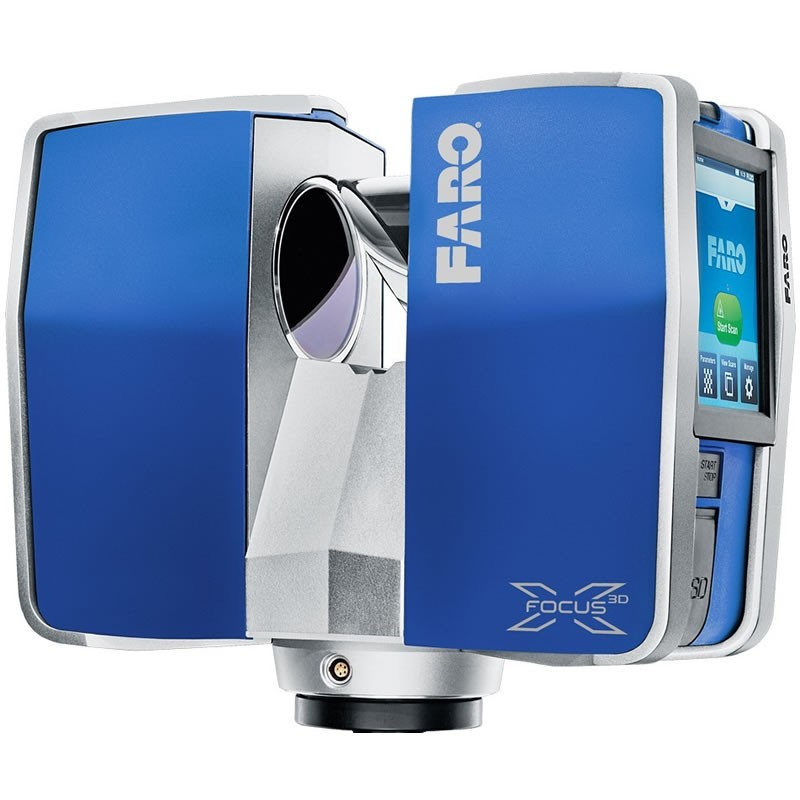
\includegraphics[height=3cm,width=\columnwidth]{figs/3dsensors/faro}
\caption{text for the first subfigure}
\label{sfig:testa}
\end{subfigure}\hfill
\begin{subfigure}{0.49\columnwidth}
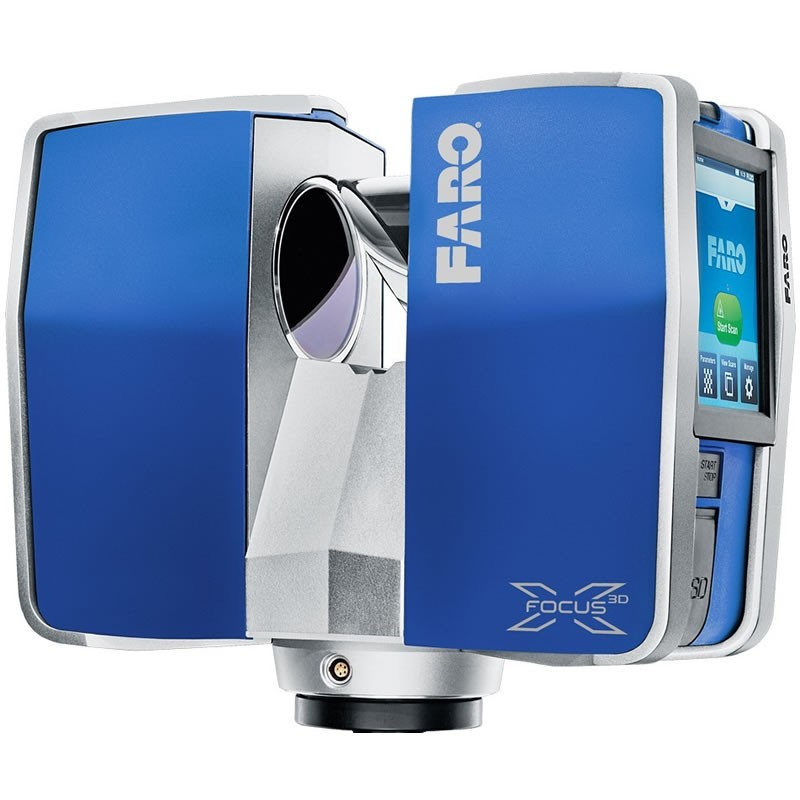
\includegraphics[height=3cm,width=\columnwidth]{figs/3dsensors/faro}
\caption{test for the second subfigure}
\label{sfig:testb}
\end{subfigure}\hfill
\caption{}
\label{}
\end{figure*}

%TODO acertar figura

\paragraph{Velodyne}

A empresa Velodyne possui, atualmente, 3 modelos de 3D Lidar. Os modelos variam
basicamente no número de pares de emissores e receptores e, consequentemente, na
resolução final. Os modelos são o VLP-16, o HDL-32E e HDL-64E, com 16,32 e 64
canais respectivamente. Esse tipo de sensor possui uma alta taxa de
atualização, entretanto não possui uma alta densidade de dados. O modelo mais
utilizado é o intermediário HDL-32E.

\begin{itemize}
\item 32 pares laser/detector  
\item Campo de Visão: +10.67$^o$ to -30.67$^o$ (vertical)
\item Rotação de $360^o$
\item Alcance - 1m - 100m 
\item 10 Hz frame rate (selecionável 5-20Hz)
\item Temperatura de Operação $-10^o$ to $+60^o$ C
\item Acurácia: $<$2 cm
\item Resolução Angular (vertical) 1.33$^o$
\item Peso: HDL-32E = 1kg; Cabos = 0.3kg
\item Tamanho: 15cm altura x 8.6cm diâmetro
\item Proteção: IP67
\item Correção de orientação (internal MEMS acelerometros and gyros)
\end{itemize}

\begin{figure}[h!]
   \centering
   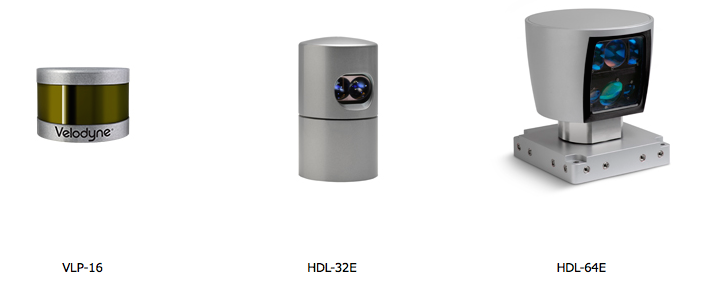
\includegraphics[width=0.8\columnwidth]{figs/3dsensors/velodyne}
   \caption{Velodyne Models}
   \label{fig::velodyne_models}
\end{figure}

\paragraph{Forecast 3D Laser System}


O sensor Forecast 3D consiste em um senor 2D laser da SICK, modelo LMS 151 ou
511, acoplado a uma unidade $pan-tilt$. O seu preço esta na faixa de
U\$37.000,00.


\begin{figure}[h!]
   \centering
   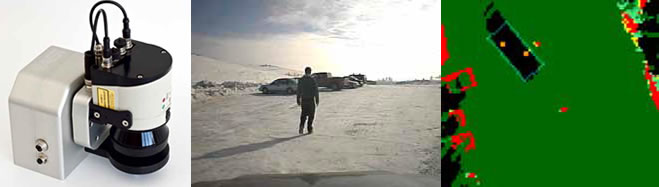
\includegraphics[width=0.8\columnwidth]{figs/3dsensors/forecast}
   \caption{Forecast 3D Laser System}
   \label{fig::forecast}
\end{figure}

\subsubsection{ToF Cameras}

Conhecidas como Time-of-Flight Cameras, são dispositivos compostos por apenas
uma câmera, não necessitando de uma configuração estéreo para triangularização
de imagens. Esse tipo de dispositivo utiliza uma fonte infra-vermelho interna e de
forma análoga aos dispositivos laser, calcula a distância a partir da diferença
de fase do sinal refletido. Entretanto, essa tecnologia possibilita o cálculo
simultâneo das distâncias de cada objeto na região iluminada pela fonte IR,
mesmo que com resoluções limitadas.

\paragraph{Mesa Imaging SwissRanger SR4000}


\begin{itemize}
  \item Alcance para detecção: 0.1 - 10.0 m
  \item Alcance calibrado: 0.8 - 8.0 m
  \item Drift com a temperatura (T) - $\leq$ 1.5 mm/$^o$C (max.) - For 10$^o$C
  $\leq$ T $\leq$ 50$^o$C
  \item Tamanho: 65 x 65 x 76 mm
  \item Peso: 510 g
\end{itemize}

\begin{figure}[h!]
   \centering
   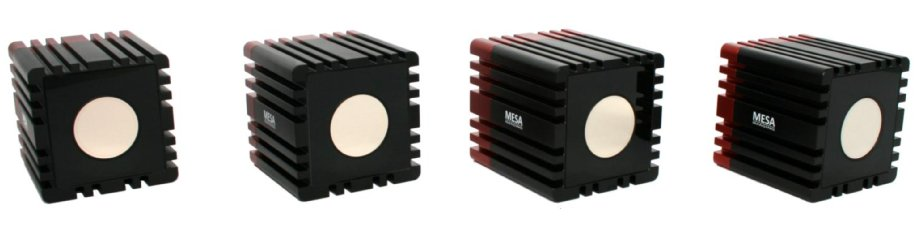
\includegraphics[width=0.8\columnwidth]{figs/3dsensors/mesa2}
   \caption{Mesa Imaging SwissRanger SR4000}
   \label{fig::mesa}
\end{figure}

\paragraph{Sentis M100 / Argos 3D - P100}

\begin{itemize}
  \item Medidas de distância e vídeo em tons de cinza
  \item Resolução: 160 x 120 pixels
  \item 40 - 160 fps
  \item Alcance: $>$3m  (extensível até 10m indoor)
  \item Campo de Visão: $90^o$
  \item Tamanho: 75 x 57 x 26 mm
  \item Peso:
\end{itemize}

\begin{figure}[h!]
   \centering
   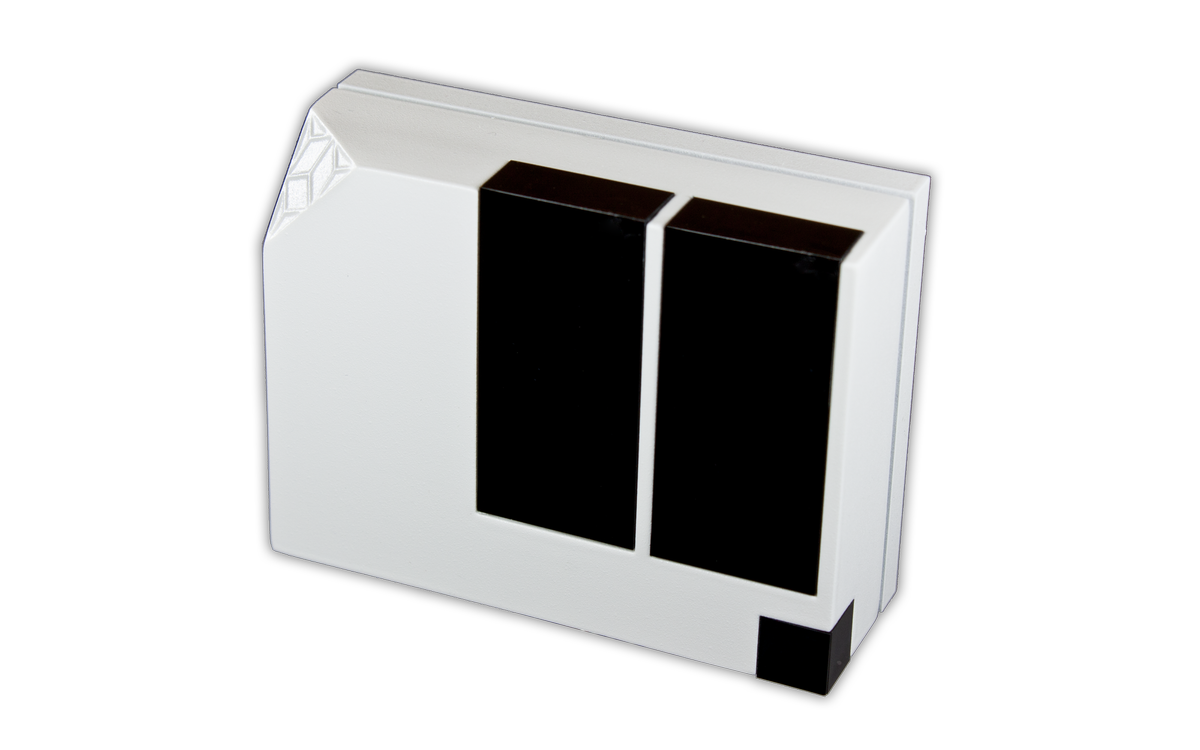
\includegraphics[width=0.8\columnwidth]{figs/3dsensors/argos3dp100}
   \caption{Sensor Argos 3D - P100}
   \label{fig::forecast}
\end{figure}

\subsubsection{Câmeras de Luz Estruturada}

Estes sensores constituem de uma fonte emissora de infra-vermelho e um receptor.
Um padrão é projetado na cena a ser reconstruida e a partir da distorção desse
padrão é possível o cálculo de distâncias. 

%TODO exemplos dos sensores de luz estruturada
%TODO Pros e cons

%TODO ELAEL - decidir se abre uma subseção d eaplicações ou coloca um exemplo de
% aplicação em cada componente - utilizar o seu material do SOTA em 3D sensors. 

\begin{center}
\begin{tabular*}{\columnwidth}{l @{\extracolsep{\fill}} cc}
\hline
{\bf Características}           & {\bf
\begin{tabular}[x]{@{}c@{}}Luz\\Estruturada\end{tabular}}                       
& {\bf ToF}                                                  \\ \hline {\bf Complexidade de Software}  & Média                                                      & \cellcolor[HTML]{92D050}{\color[HTML]{000000} {\bf Baixa}} \\
{\bf Custo Material}            & \cellcolor[HTML]{FE0000}{\color[HTML]{FFFFFF} {\bf Alto}}  & Médio                                                      \\
{\bf Tamanho}                   & Grande                                                     & \cellcolor[HTML]{92D050}{\bf Pequeno}                      \\
{\bf Tempo de Resposta}         & \cellcolor[HTML]{FE0000}{\color[HTML]{FFFFFF} {\bf Alto}}  & \cellcolor[HTML]{92D050}{\bf Baixo}                        \\
{\bf Acurácia da Profundidade}  & \cellcolor[HTML]{92D050}{\bf Alta}                         & Média                                                      \\
{\bf Qualidade com Pouca Luz}  & \cellcolor[HTML]{92D050}{\bf Boa}                          & \cellcolor[HTML]{92D050}{\bf Boa}                          \\
{\bf Qualidade com Muita Luz} & \cellcolor[HTML]{FE0000}{\color[HTML]{FFFFFF}
{\bf Fraca}} & \cellcolor[HTML]{92D050}{\bf Boa}                          \\
{\bf Consumo de Energia}        & Médio                                                      & \cellcolor[HTML]{92CDDC}{\bf Escalavel}                    \\
{\bf Alcance}                   & \cellcolor[HTML]{92CDDC}{\bf Escalavel}                    & \cellcolor[HTML]{92CDDC}{\bf Escalavel}                    \\ \hline
\end{tabular*}
\captionof{table}{Comparativo Luz Estruturada vs ToF. Fonte: \citep{larrylitof}}
%\caption{Dados principais do processo de metalização HVOF}
\label{tab::estructvstof}
\end{center}

\subsection{Conclusão}

As restrições apresentadas pelo problema de calibração, dentro do ambiente da
turbina, impõem um conjunto de requisitos mínimos que o sensor deve apresentar:

\begin{itemize}
  \item Alta resolução
  \item Portabilidade
  \item Alcance suficiente (>20m)
  \item Resistir as condições de temperatura e umidade 
\end{itemize}

Além desses requisitos, é desejável também que o sensor tenha alimentação
idependente e que sua velocidade de escaneamento não seja um fator limitante
para a eficiência do processo.

A classe de sensores que atende todas essas condições é a das Estações de
medição, com exceção do sensor Nikon MV 330 que não possui a portabilidade
necessária para a solução proposta, além de ter um preço muito maior que de seus
concorrentes.

O sensor Faro Focus X330, além de satisfazer os requisitos mínimos, é o que
possui menor preço e, por isso, foi escolhido como o o sensor a ser utilizado na
calibração do sistema e reponsável por colher os dados espacias do ambiente da
turbina e do robô. 

Entretanto, pelas especificações do sistema não foi possível garantir a perfeita
operação do sensor nas condições de alta umidade apresentada no interior da
turbina. O dipositivo opera com um sistema de lentes e lasers e, caso apresente
condensação em um desses componentes, o resultado final de sensoriamento pode
ser prejudicado. Devido a este fato, foi realizado uma bateria de testes na
Usina de Jirau, no interior de uma turbina, afim de confirmar a viabilidade
técnica desse sensor.

O teste realizado constituiu na utlização de quatro esferas reflexivas,
representadas na figura \ref{fig::esferas}, distribuidas pelo ambiente da
turbina.
Em seguida, foram realizadas 4 coletas de dados, sendo 3 delas à jusante do
rotor e uma entre as pás do rotor e o distribuidor. Com a nuvem de pontos
coletada, foi possível utilizar a assinatura única gerada pelas esferas para
alinhar todos os conjuntos de dados em uma única imagem 3D.

\begin{figure}[h!]
\centering
	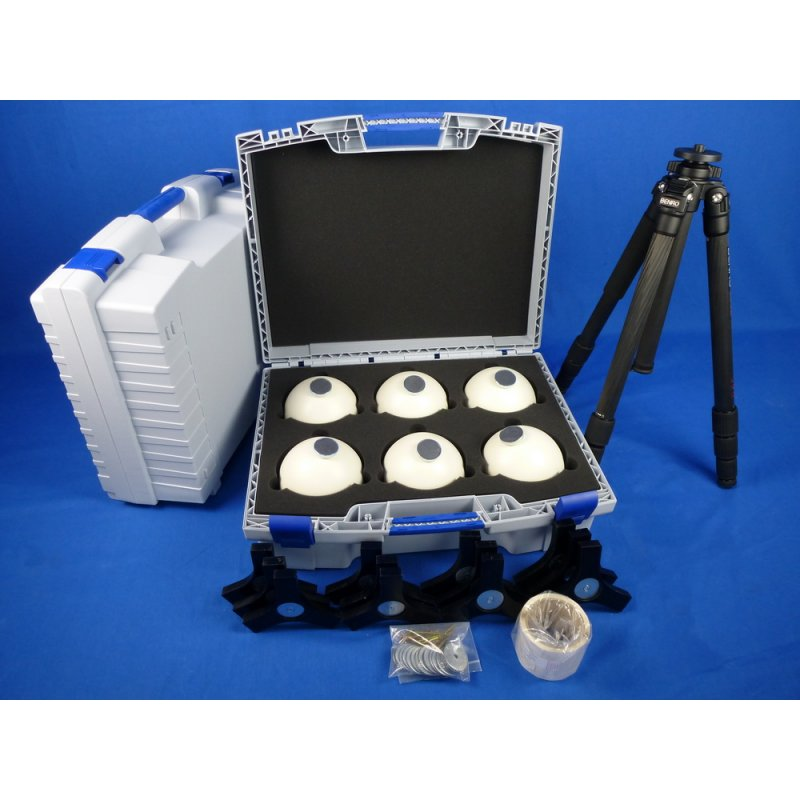
\includegraphics[width=0.9\columnwidth]{figs/3dsensors/kit}
	\caption{Conjunto de esferas reflexivas e tripé}
	\label{fig::esferas}
\end{figure}

A figura \ref{fig::turbina_faro} representa a vista frontal da imagem gerada e, por sua
vez, a figura \ref{fig::turbina_cad} representa uma reconstrução 3D gerada a
partir da nuvem de pontos coletas e utilizando o software proprietário do
fornecedor do sensor. 

\begin{figure}[h!]
\centering
	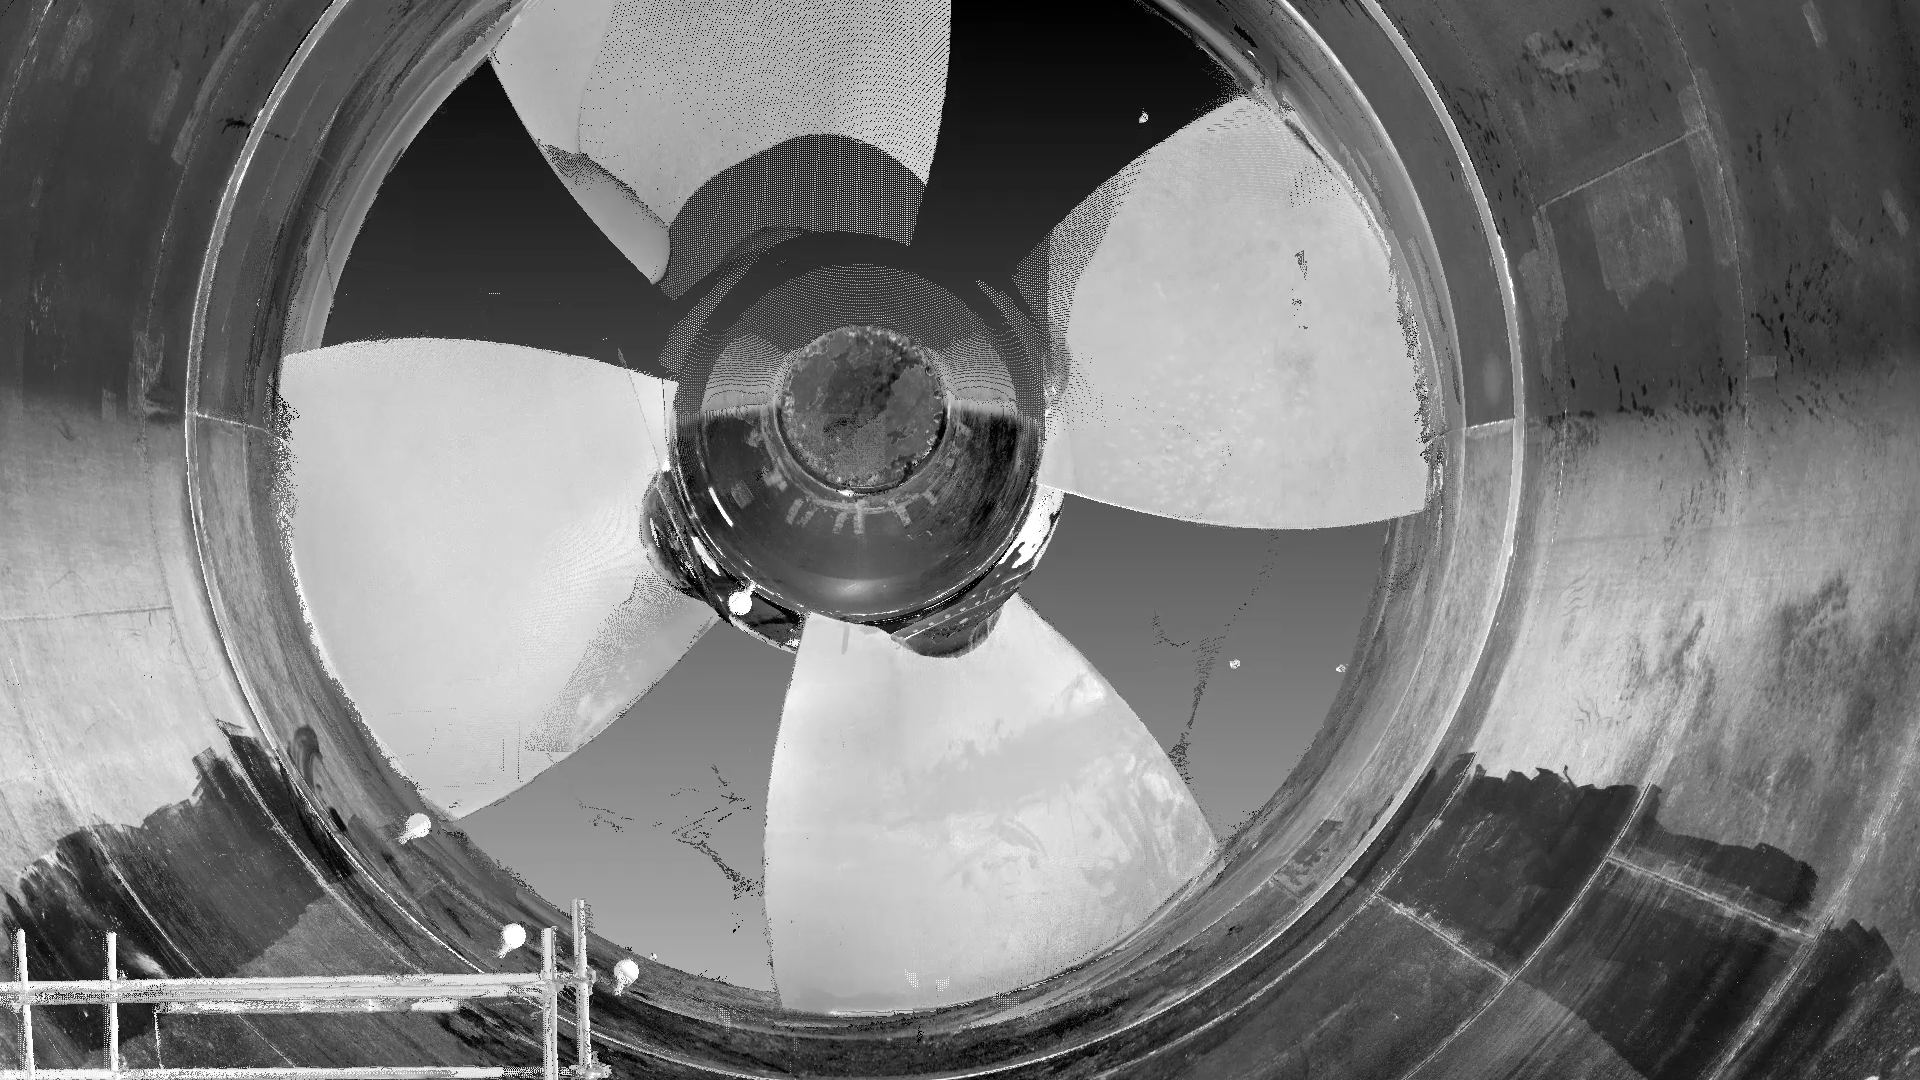
\includegraphics[width=0.9\columnwidth]{figs/3dsensors/recorte_video}
	\caption{Vista frontal da imagem gerada a partir dados adquiridos durante o
	teste.}
	\label{fig::turbina_faro}
\end{figure}

\begin{figure}[h!]
\centering
	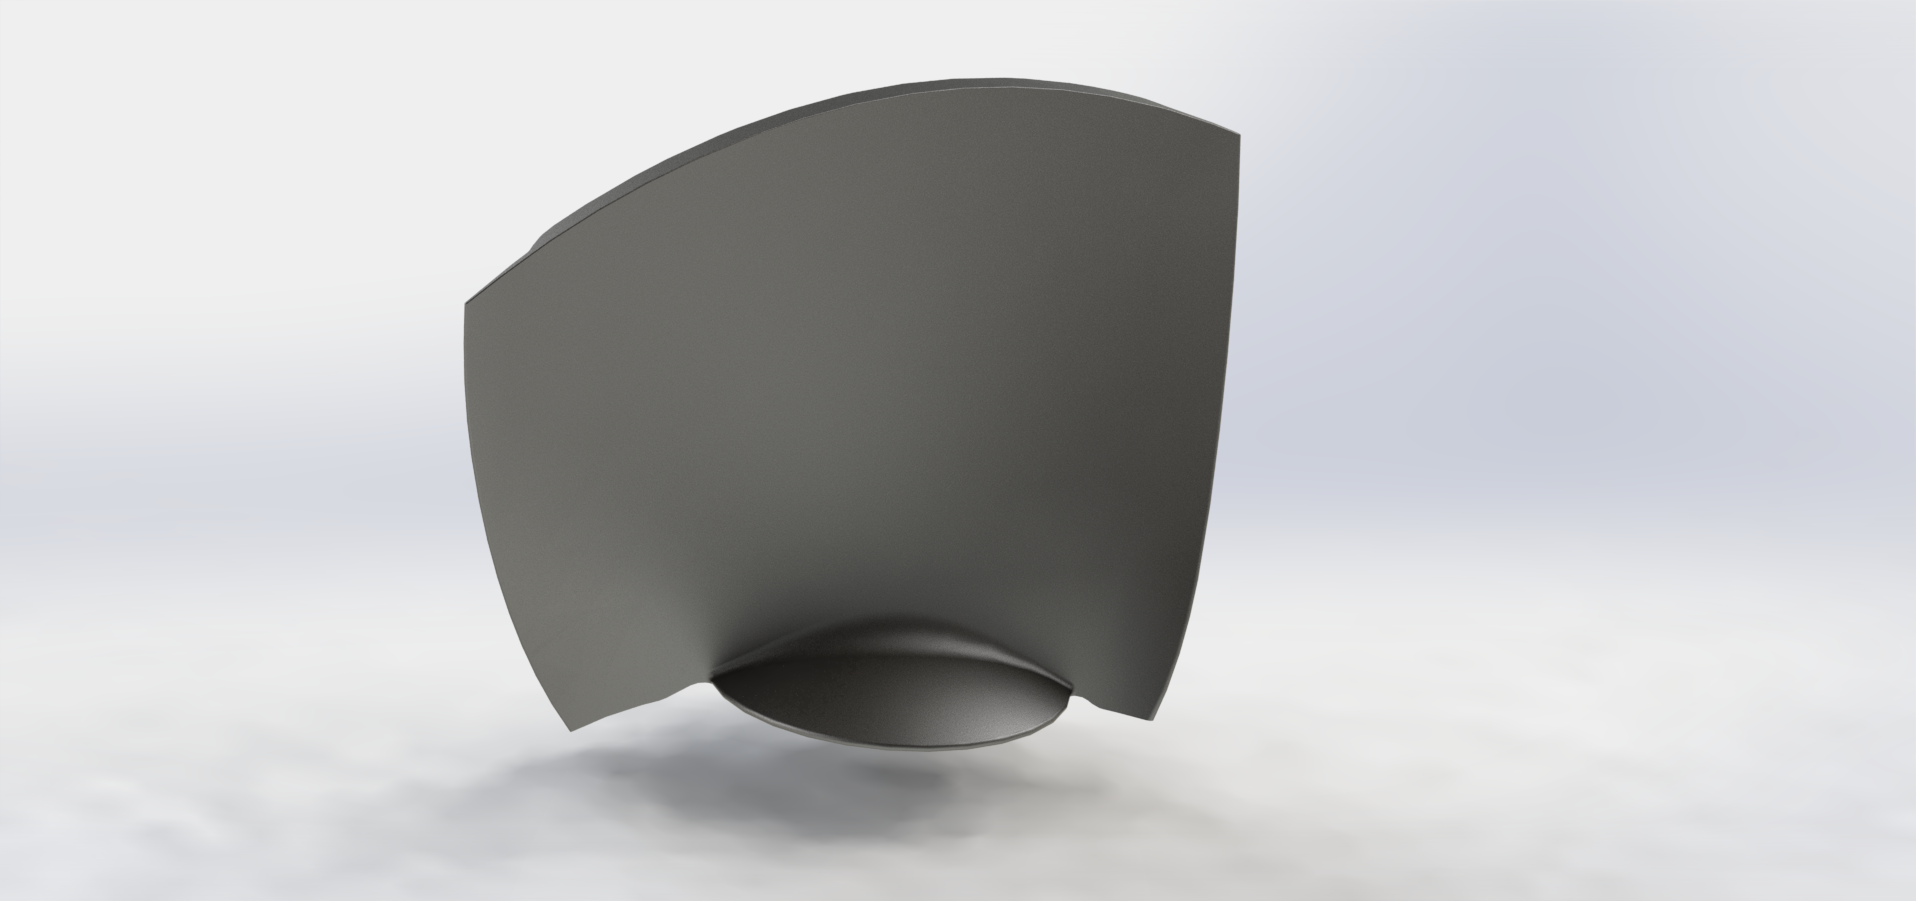
\includegraphics[width=0.9\columnwidth]{figs/3dsensors/Pa_Real_Render_04}
	\caption{Reconstrução em CAD da pá com os dados do teste.}
	\label{fig::turbina_cad}
\end{figure}

A partir dos resultados gerados durante os testes foi comprovada que o sensor é
capaz de operar nas condições extremas impostas pela turbina e com um nível de
ruído aceitável para a aplicação em questão. 


\subsubsection{Medidor de distância a Laser}

Durante o processo de metalização o 3D scanner estará desligado, pois o tempo de
varedura não o torna prático para obter informações em tempo real. Assim o
sistema estaria funcionando em \textit{loop} aberto, o que gera receios com
relação à segurança. A fim de evitar tais riscos é desejável alguma
realimentação para o sistema sobre sua posição. Essa realimentação será
realizada pelo uso de um medidor de distância a Laser, a ser posicionado próximo
à pistola de metalização, com o intuito de aferir a distância da pistola até a
pá em tempo real.

\begin{figure}[h!]
\centering
	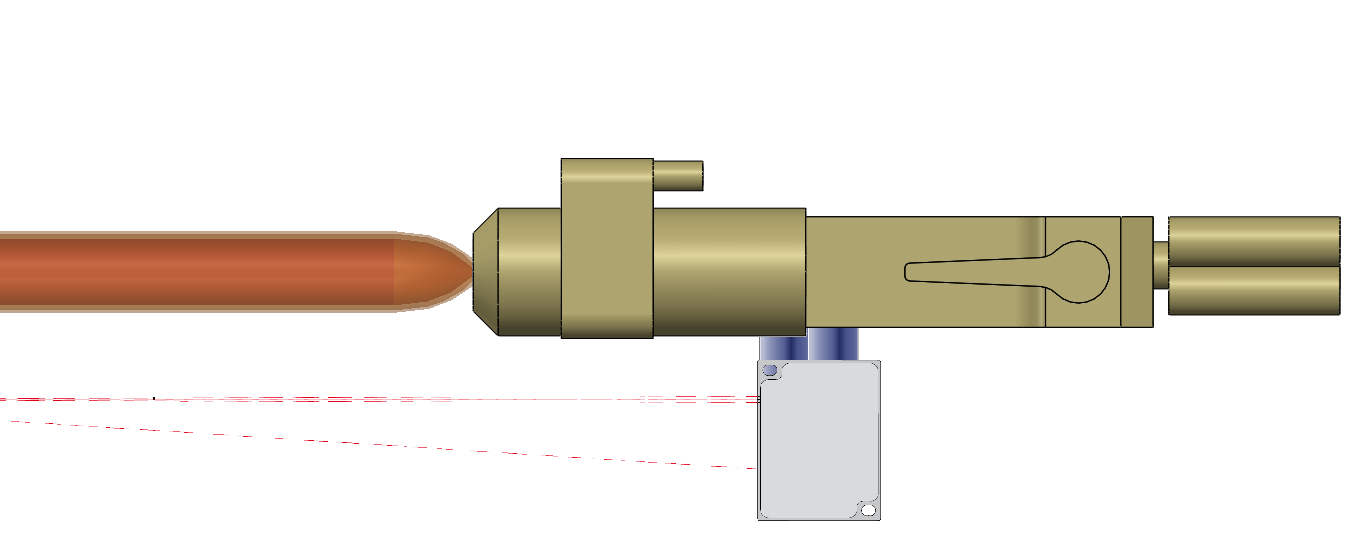
\includegraphics[width=0.9\columnwidth]{figs/3dsensors/senso_laser_pistola}
	\caption{Ilustração da posição do medidor de distância, em cinza, na pistola de
	metalização.}
	\label{fig::laser}
\end{figure}


Para a escolha de medidor compatível foram analisadas as seguintes variáveis:

\paragraph{Temperatura}
A temperatura da superfície pode influenciar na precisão do sensor devido à
radiação de corpo negro. Caso essa radiação térmica atinja níveis relevantes na
faixa de frequência do Laser utilizado ocorre degradação da qualidade de
reposta do sensor. Análises de campo identificaram que, apesar da alta
temperatura da chama de metalização, a pá da turbina não chega a emitir níveis
preocupantes de radiação na faixa do vermelho ($670 nm$), onde operam os Lasers
padrões. Para casos de exceção existem Laser que trabalham em regiões do
azul/violeta.

Por outro lado a temperatura do ambiente também influencia o sensor, que não
costuma ter alta resistência à temperatura, ficando algo em torno do $50^oC$.
Para evitar que o calor da chama seja recebido diretamente pelo sensor,
aumentando a temperatura ambiente na região, ele deve ser posicionado na pistola
com uma distância de segurança da chama (figura \ref{fig::laser}).

\paragraph{Distância de operação}
A metalização ocorre com a pistola entre 23cm e 24cm de distância da pá. Somado
a isso temos a distância do sensor à chama para então sabermos a distância da
pá ao sensor. Considerando que a pistola possui em torno de 30cm de comprimento,
a faixa de operação de distâncias do sensor deverá incluir 40-50cm. Para termos
essa região no centro da faixa de operação, ela deverá iniciar em 20-25cm e
trabalhar até 80-100cm.

\paragraph{Poeira e Umidade}
A alta umidade ambiente dentro do aro câmara, e em todo circuito hidráulico,
impõe mais um requisto sobre o equipamento. Além disso, o pó residual da
aplicação da metalização pode ser danoso ao sensor. Um isolamento apropriado
para o sensor pode ser encontrado segundo a padronização IP69K.

\paragraph{Precisão}
Como a tolerância está na ordem de milímetros ( a distância do sensor à pá deve
se manter em uma faixa de $\pm 5mm $ entre 23cm e 24cm ), logo é desejável que o
sensor possua precisão de $1mm$ ou menor.

\paragraph{Peso}
Considerando a carga máxima no punho do robô de 10kg, e a massa da pistola de
8,5kg e aplicando as restrições dinâmicas ( para manter a velocidade
desejada em todos os pontos ) conclui-se que o medido deve ter uma massa
inferior a 1kg.


